\section{Introduction}

\subsection{Sunway TaihuLight}
\begin{frame}
    \frametitle{Sunway TaihuLight}
	\begin{itemize}
		\item A supercomputer that ranks the first in the world.
		\item Over 100 Pflops computing capacity. 
		\item Sunway TaihuLight is power by a new SW26010 many-core processor.  
		\item Not only the fastest but also the greenest supercomputer in the world.  
	\end{itemize} 
\end{frame}

\subsection{SW26010}
\begin{frame}
    \frametitle{SW26010}
	\begin{itemize}
		\item Peak double-precision performance of 3.06 Tflops.
		\item 300 watts power consumption.
		\item Combine both management cores and computing core clusters on a core group.  
		\item Support a user-controlled fast buffer for each computing cores. 
		\item Rigister communication between computing cores.
		\item Each computing core consists of two execution pipelines.  
	\end{itemize} 
\end{frame}

\subsection{Convolution layer}
\begin{frame}
    \frametitle{Convolution layer}
	\begin{figure}
		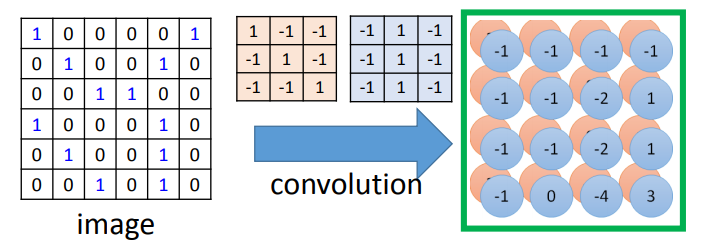
\includegraphics[scale=0.5]{figure/conv-1.PNG}
	\end{figure}
\end{frame}

\begin{frame}
    \frametitle{Convolution layer}
	\begin{figure}
		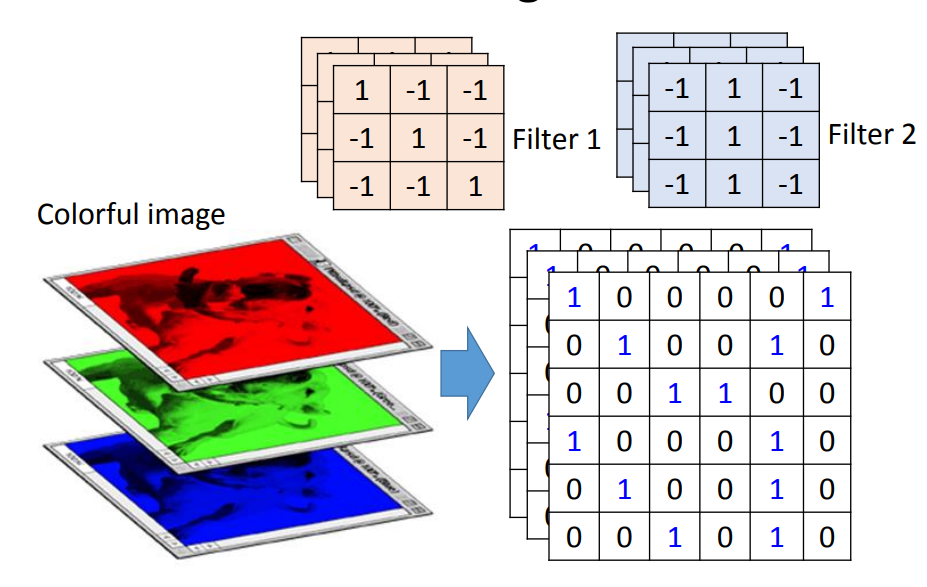
\includegraphics[scale=0.4]{figure/conv-2.PNG}
	\end{figure}
\end{frame}

\begin{frame}
    \frametitle{Peseudo code of a convolutional layer}
	\begin{figure}
		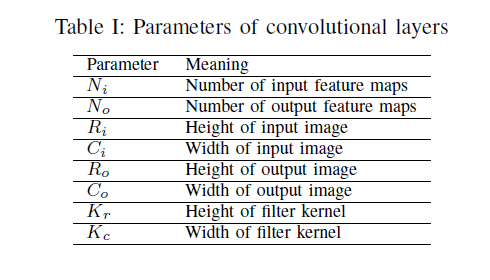
\includegraphics[scale=0.6]{figure/variable.PNG}
	\end{figure}
\end{frame}

\begin{frame}
	\frametitle{Pseudo code of a convolutional layer}
	for $cB$ = 0 to B\\
	\hspace{0.2cm}for $cR_{o}$ = 0 to $R_{o}$\\
	\hspace{0.4cm}for $cC_{o}$ = 0 to $C_{o}$\\
	\hspace{0.6cm}for $cN_{o}$ = 0 to $N_{o}$\\
	\hspace{0.8cm}for $cK_{r}$ = 0 to $K_{r}$\\
	\hspace{1cm}for $cK_{c}$ = 0 to $K_{c}$\\
	\hspace{1.2cm}for $cN_{i}$ = 0 to $N_{i}$\\
	\hspace{1.4cm}out$[cB][cR_{o}][cC_{o}][cN_{o}]$ +=\\
	\hspace{1.4cm}in$[cB][cR_{o}+cK_{r}][cC_{o}+cK_{c}][cN_{i}]$*filter$[cN_{o}][cK_{r}][cK_{c}][cN_{i}]$
		
\end{frame}

\begin{frame}
	\frametitle{General Matrix-Multiplication(GEMM)}
	\begin{figure}
		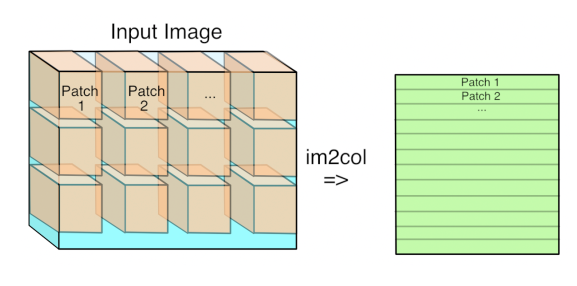
\includegraphics[scale=0.5]{figure/imtocol.PNG}
	\end{figure}
\end{frame}

\begin{frame}
	\frametitle{GEMM}
	\begin{figure}
		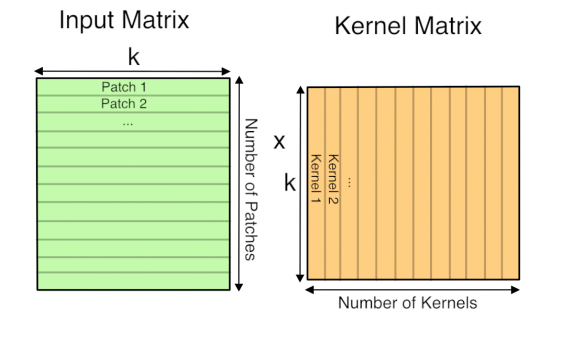
\includegraphics[scale=0.5]{figure/gemm.PNG}
	\end{figure}
\end{frame}

